\section{F0: Does the Reward Bit Change Written Memory?}
\label{sec:f0}
We test the write channel with a paired intervention over released Salesforce trajectories. The source parquet contains task prompts and full action histories from the published WebArena runs. We select six trajectories through a deterministic rule that balances original outcomes. Three trajectories originally receive benchmark success. Three originally receive benchmark failure.

For every trajectory, we construct two ReasoningBank memory prompts. The first uses the released success-reflection system prompt. The second uses the released failure-reflection system prompt. The task text and action history are copied byte-for-byte into both conditions. DeepSeek-V4-Flash writes the paired memories at temperature zero. Provider responses are archived before analysis through content-addressed raw receipts.

Four trajectory pairs return complete memory outputs in both intervention arms. Every complete pair changes the normalized memory content. Every complete pair also changes the extracted memory-item title set. Token-set Jaccard distance ranges from 0.691 to 0.770. The mean distance is 0.735. Table~\ref{tab:f0} reports the pair-level values.

\begin{table}[t]
\centering
\caption{Paired memory divergence under the reward-label intervention.}
\label{tab:f0}
\small
\begin{tabular}{lcc}
\toprule
Task ID & Original outcome & Token Jaccard distance \\
\midrule
21 & failure & 0.691 \\
22 & failure & 0.708 \\
23 & success & 0.770 \\
25 & success & 0.770 \\
\bottomrule
\end{tabular}
\end{table}

\begin{figure}[t]
\centering
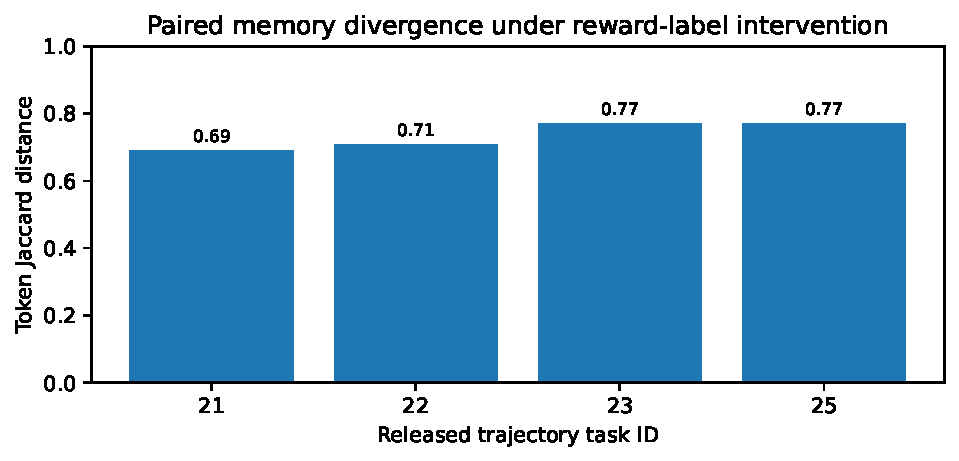
\includegraphics[width=0.95\linewidth]{figures/fig2_f0_memory_divergence.pdf}
\caption{The same released trajectory produces different persistent memories when the reward-conditioned reflection mode is flipped.}
\label{fig:f0}
\end{figure}

The intervention changes more than surface phrasing. For task 21, the success writer produces guidance centered on opening the review section and preserving direct quotes. The failure writer emphasizes exhaustive pagination and extraction verification. Task 23 shows a similar causal split. The success writer highlights evidence collection across pages. The failure writer focuses on pagination state and broader synonym coverage. The trajectory supplied to both writers is identical in each pair.

The result survives the F0 falsifier. Reward-conditioned memory writing is a real state channel in the released implementation. The effect appears in both original-outcome strata, which rules out a simple explanation based on selecting only trajectories that already failed.

This establishes the first stage of the paper mechanism:
\begin{equation}
\text{reward label}\longrightarrow\text{memory content}.
\end{equation}
The next experiment tests the second stage by injecting the paired memories into matched future tasks.
